\chapter{Crypto.Symmetric.MAC}\label{MAC}
A message authentication code (MAC) ensures the integrity of a message
and sender authentication. It uses a symmetric key (RMAC uses two
symmetric keys). The result of the MAC is named an authentication
tag. The developer of this library marks it as a (digital)
stamp. Three MACs are provided in the ACL, they are randomized MAC
(RMAC), hash function based MAC (HMAC) and cipher-based MAC (CMAC).

%%%%%%%%%%%%%%%%%%%%%%%%%%%%%%%%%%%%%%%%%%%%%%%%%%%%%%%%%%%%%%%%%%
%%%%%%%%%%%%%%%%%%%%%%%%%%%%%%%%%%%%%%%%%%%%%%%%%%%%%%%%%%%%%%%%%%

\section{Randomized MAC (RMAC)}
RMAC is developed by Eliane Jaulmes, Antoine Joux and Frederic
Valette. It is based on CBC-MAC and one-way block cipher (Chapter
\ref{Oneway-Blockcipher}). It is proved save against the birthday
attack. Two keys are required in RMAC.

 Mathematical description: $RMAC_{K_1,K_2}(E,M)=E_{K_2\oplus
   R}(C_n)$\,, with $C_i=E_{K_1}(M_i\oplus C_{i-1})$,
 $R\in_R\{0,1\}^{|K_1|}$ and $C_0=0^n$.

\subsubsection*{Generic Part}
\begin{lstlisting}{}
  generic
    with package C is new
    					Crypto.Symmetric.Oneway_Blockcipher(<>);
    with procedure Read (Random : out C.Key_Type) is <>;
    with function "xor" (Left, Right : C.Block) return C.Block is <>;
    with function "xor" (Left, Right : C.Key_type)
     							return C.Key_Type is <>;
\end{lstlisting}

\subsubsection*{High-Level-API}
\begin{lstlisting}{}
  type Blocks  is array (Integer range <>) of Block;
  procedure Sign(Message    : in Blocks;
                 Key1, Key2 : in Key_Type;
                 R          : out Key_Type;
                 Tag        : out Block);
  function Verify(Message    : in Blocks;
                  Key1, Key2 : in Key_Type;
                  R          : in Key_Type;
                  Tag        : in Block)  return Boolean;
\end{lstlisting}
The procedure \texttt{Sign()} signs \texttt{Message} with two keys,
Key1 and Key2. The message is delivered as an array of blocks. Key1 is
used to encrypt the whole message blocks, and Key2 is used to generate
the final tag based on the calculated ciphertext.

The function \texttt{Verify()} returns true if the term \texttt{Tag}
is a valid stamp, otherwise it returns false. When one or more
parameters don't agree with those generated from the procedure
\texttt{Sign()}, then the function returns false with a significant
probability.


\subsubsection*{Low-Level-API}
\begin{lstlisting}{}
  procedure Init(Key1, Key2    : in Key_Type);
  procedure Sign(Message_Block : in Block);
  procedure Final_Sign(Final_Message_Block : in Block;
                       R    : out Key_Type;
                       Tag  : out Block);
  procedure Verify(Message_Block : in Block);
  function Final_Verify(Final_Message_Block : in Block;
                        R   : in Key_Type;
                        Tag : in Block)   return Boolean;
\end{lstlisting}
\begin{itemize}
\item The procedure \texttt{Init()} initializes RMAC with two keys,
  and sets an internal initial state.
\item The procedure \texttt{Sign()} encrypts a message block
  (\texttt{Message\_Block}). Every time it works only on one block, if
  there are blocks more than one, the procedure should be called til
  the last block.
\item The procedure \texttt{Final\_Sign()} encrypts the last message
  block \texttt{Final\_Message\_Block}, and then generates a random
  number $R$ to calculates the stamp $Tag$, and finally resets RMAC.
\item The procedure \texttt{Verify()} encrypts a message block
  (\texttt{Message\_Block}). Every time it works only on one block.
\item The function \texttt{Final\_Verify()} decrypts the last message
  block \texttt{Final\_Message\_Block}, calculates a new tag and then
  compares the tag with the delivered one to test if it is valid. True
  is returned if valid, otherwise false.
\end{itemize}

\subsubsection*{Example}
\begin{lstlisting}{}
  with Crypto.Types; use Crypto.Types;
  with Ada.Text_IO; use Ada.Text_IO;
  with Crypto.Types.Random; use Crypto.Types.Random;
  with Crypto.Symmetric.MAC.RMAC;
  with Crypto.Symmetric.Oneway_Blockcipher_AES128;
  pragma Elaborate_All(Crypto.Symmetric.MAC.RMAC);
  procedure Example_RMAC is
   package AES128 renames Crypto.Symmetric.Oneway_Blockcipher_AES128;
    package RMAC128 is new Crypto.Symmetric.MAC.RMAC(AES128);
    use RMAC128;
    Key1: B_Block128:= (16#00#, 16#01#, 16#02#, 16#03#, 16#04#,
                        16#05#, 16#06#, 16#07#, 16#08#, 16#09#,
                        16#0a#, 16#0b#, 16#0c#, 16#0d#, 16#0e#,
                        16#0f#);
    Key2 : B_Block128:=(16#00#, 16#11#, 16#22#, 16#33#, 16#44#,
                        16#55#, 16#66#, 16#77#, 16#88#, 16#99#,
                        16#aa#, 16#bb#, 16#cc#, 16#dd#, 16#ee#,
                        16#ff#);
    R, Tag : B_Block128;
    M : String :="All your base are belong to us! ";
    Message : RMAC128.Blocks(0..1) :=
                        (To_B_Block128(To_Bytes(M(1..16))),
                         To_B_Block128(To_Bytes(M(17..32))));
  begin
     -- Low-Level
    Init(Key1, Key2);
  	 Sign(Message(0));
  	 Final_Sign(Message(1), R, Tag);
 	 Init(Key1, Key2);
  	 Verify(Message(0));
  	 Put_Line(Final_Verify(Message(1), R, Tag)'Img);
  end Example_RMAC;
\end{lstlisting}

%%%%%%%%%%%%%%%%%%%%%%%%%%%%%%%%%%%%%%%%%%%%%%%%%%%%%%%%%%
%%%%%%%%%%%%%%%%%%%%%%%%%%%%%%%%%%%%%%%%%%%%%%%%%%%%%%%%%%

\section{Hash-based MAC (HMAC)}
The designers of HMAC are Mihir Bellare, Ran Canettiy and Hugo
Krawczykz. It is based on a hash function. In addition, HMAC\_SHA1,
HMAC\_SHA256, HMAC\_512 and HMAC\_Whir\-lpool are
available.

Mathematical description: $HMAC_K(H,M)=H(K\oplus opad,H((K\oplus
ipad)||M))$\,, with $opad=\{0x5C\}^n$ and $ipad=\{0x36\}^n$.

\subsubsection*{Generic Part}
\begin{lstlisting}{}
  generic
    with package H is new Crypto.Symmetric.Hashfunction(<>);
    with function "xor"(Left, Right : H.Message_Type)
      					          return H.Message_Type is <>;
    with procedure Fill36 (Ipad : out  H.Message_Type) is <>;
    with procedure Fill5C (Opad : out  H.Message_Type) is <>;
    with procedure Copy (Source : in  H.Hash_Type;
      					    Dest   : out H.Message_Type) is <>;
\end{lstlisting}
The two procedures \texttt{Fill36()} and \texttt{Fill5C()} make the
outer/inner padding with value $0x36$ or $0x5C$.  The procedure
\texttt{Copy()} copies the content of \texttt{Source} to
\texttt{Dest}. If the size of the source value is smaller than that of
the destination value, then the rest will be padded with zeros.  All
these helping operations are defined in
\texttt{Crypto.Symmetric.MAC}.

\subsubsection*{API}
\begin{lstlisting}{}
  procedure Init(Key : in Message_Type);
  procedure Sign(Message_Block : in Message_Type);
  procedure Final_Sign
      (Final_Message_Block        : in Message_Type;
       Final_Message_Block_Length : in Message_Block_Length_Type;
       Tag                        : out Hash_Type);
  procedure Verify(Message_Block : in Message_Type);
  function Final_Verify
      (Final_Message_Block        : Message_Type;
       Final_Message_Block_Length : Message_Block_Length_Type;
       Tag                        : Hash_Type) return Boolean;
\end{lstlisting}
\begin{itemize}
\item Procedure \texttt{Init()} initializes the \texttt{HMAC} with the
  key and sets an initial state.
\item Procedure \texttt{Sign()} hashs a message block
  (\texttt{Message\_Block}). It is called until to the second to last
  block.
\item Procedure \texttt{Final\_Sign()} hashs the last message block of
  the length \texttt{Final\_Message\_B\-lock\_Length}, returns a
  digital stamp tag and resets the HMAC.
\item Procedure \texttt{Verify()} hashs a message block.
\item The function \texttt{Final\_Verify()} hashs the last message
  block of the length \texttt{Final\_Message\_B\-lock\_Length}, then
  verifies whether the tag is valid or not. It returns true if valid,
  else false.
\end{itemize}

\subsubsection*{Example}
\begin{lstlisting}{}
  with Crypto.Types;
  with Ada.Text_IO;
  with Crypto.Symmetric.MAC;
  with Crypto.Symmetric.MAC.HMAC;
  with Crypto.Symmetric.Hashfunction_SHA256;
  use Crypto.Types;
  use Ada.Text_IO;
  pragma Elaborate_All(Crypto.Symmetric.MAC.HMAC);
  procedure Example_HMAC is
    package HMAC256 is new Crypto.Symmetric.MAC.HMAC
				      (H =>Crypto.Symmetric.Hashfunction_SHA256,
		    		 	 Copy =>Crypto.Symmetric.MAC.Copy,
						 Fill36 =>Crypto.Symmetric.MAC.Fill36,
						 Fill5C =>Crypto.Symmetric.MAC.Fill5C);
    use HMAC256;
    Key : W_Block512 :=(0 => 16#0b0b0b0b#, 1 => 16#0b0b0b0b#,
		                  2 => 16#0b0b0b0b#, 3 => 16#0b0b0b0b#,
		                  4 => 16#0b0b0b0b#, others => 0);
    Message : W_Block512 :=(0 => 16#48692054#, 
    								 1 => 16#68657265#, others => 0);
    Tag : W_Block256;
  begin
    Init(Key);
    Final_Sign(Message, 8, Tag);
    Put_Line(Final_Verify(Message, 8, Tag)'Img);
  end Example_HMAC;
\end{lstlisting}


\subsection*{Remark:}
The users don't need to generate a new HMAC every time. There are
already HMACs defined in the ACL.
\begin{itemize}
\item \texttt{Crypto.Symmetric.Mac.Hmac\_SHA1}
\item \texttt{Crypto.Symmetric.Mac.Hmac\_SHA256}
\item \texttt{Crypto.Symmetric.Mac.Hmac\_SHA512}
\item \texttt{Crypto.Symmetric.Mac.Hmac\_Whirlpool}
\end{itemize}
\section{Cipher-based MAC (CMAC)}
CMAC is a blockcipher-based message authentication code. It is used to
assure authenticity and integrity of the data.  CMAC is a OMAC1
described in \cite{DBLP:conf/fse/2003}. As shown in Figure \ref{OMAC},
the message is devided into blocks $m_1,m_2,\cdots,m_r$\,, and the
first $r-1$ blocks will be processed in a signature algorithm
iteratively. The intermediate values are $t_1,t_2,\cdots,
t_{r-1}$. Each round can be described mathematically as:
\begin{equation*}
t_i=E_k(t_{i-1}\oplus m_i), \quad 1\leq i \leq r-1\,,\,\mbox{and $t_0$ is a zero block}\,.
\end{equation*}
For the last message block, if it is a full block, then:
\begin{equation*}
Tag=E_k(t_{r-1}\oplus m_r \oplus U)\,,
\end{equation*}
if the block is not a full block, then it will be padded with a one bit and zero bits until it is full, and then:
\begin{equation*}
Tag=E_k(t_{r-1}\oplus m_r \oplus U_2)\,.
\end{equation*}
The terms $U$ and $U_2$ are two non-zero constants based on $L$ in the
Galois field $GF(2^n)$, where $L=E_k(0^n)$. A function is used to
calculate $U$ from $L$, and $U_2$ from $U$. It is satisfied that
$U\neq U_2$, otherwise, for a full block $m=m'10^*$ and a not full
block $m'$, after padding the second block becomes $m'10^*$, they will
lead to two identical tags, which is against our design purpose.
Details about this function can be found in \cite{DBLP:conf/fse/2003}.
\begin{figure}[h]
\centering
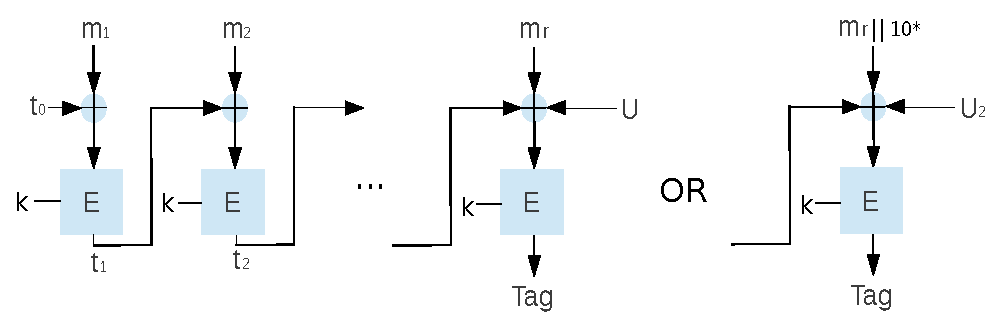
\includegraphics[scale=0.8]{./images/CMAC}
\caption{The workflow of the CMAC.}\label{OMAC}
\end{figure}


\subsubsection*{Generic Part}
\begin{lstlisting}{}
  generic
   with package C is new
   					Crypto.Symmetric.Oneway_Blockcipher(<>);
   with function To_Block_Type (B : Bytes) return C.Block;
   with function To_Bytes (B : C.Block) return Bytes;
   with function Shift_Left (Value : C.Block;
   								  Amount: Natural) return C.Block;
   with function "xor" (Left, Right : C.Block) return C.Block is <>;
\end{lstlisting}

\subsubsection*{High-Level-API}
\begin{lstlisting}{}
  type Blocks is array (Integer range <>) of Block;
  procedure Sign(Message : in  Blocks;
                 Key     : in  Key_Type;
                 Tag     : out Block);
  function Verify(Message : in Blocks;
                  Key     : in Key_Type;
                  Tag     : in Block) return Boolean;
\end{lstlisting}
Procedures and functions of high-level use the functions in
low-level. Users should always use the high-level interfaces. The
message is signed block by block calling internally low-level
functions. The function \texttt{Verify()} returns true if the newly
created tag equals the delivered tag, else false is
returned.\\

\noindent\textbf{Exception:} The terms $U$ and $U_2$ (as marked in
Figure \ref{OMAC}) are designed in 8 bytes or 16 bytes, which depends
on the block size. If the block size is neither 64 bits nor 128
bits:\quad\texttt{Blocklength\_Not\_Supported}.

\subsubsection*{Low-Level-API}
\begin{lstlisting}{}
  procedure Init(Key : in Key_Type); procedure Sign(Message_Block : in
  Block); procedure Final_Sign(Final_Message_Block : in Block;
  Bytes_Read : in Natural; Tag : out Block); procedure
  Verify(Message_Block : in Block); function
  Final_Verify(Final_Message_Block : in Block; Bytes_Read : in
  Natural; Tag : in Block) return Boolean;
\end{lstlisting}
\begin{itemize}
\item Procedure \texttt{Init()} makes initialization of the CMAC.
\item Procedure \texttt{Sign()} encrypts one message block
  (\texttt{Message\_Block}).
\item Procedure \texttt{Final\_Sign()} encrypts the last message block
  \texttt{Final\_Message\_Block}. If \texttt{Bytes\_Read} of the last
  message block isn't equal $Block'Size/8$, then it makes padding. A
  tag is generated and the CMAC is reset.
\item Procedure \texttt{Verify()} encrypts a message block. The block
  is processed as in procedure \texttt{Sign()}.
\item Procedure \texttt{Final\_Verify()} encrypts the last message
  block, and makes comparison of a newly generated tag with the
  delivered tag. It returns true if the two tags are equal, else
  false.
\end{itemize}

\noindent\textbf{Example}
\begin{lstlisting}{}
  with Ada.Text_IO; use Ada.Text_IO;
  with Crypto.Types; use Crypto.Types;
  with Crypto.Symmetric.Oneway_Blockcipher_AES128;
  with Crypto.Symmetric.MAC.CMAC;
  pragma Elaborate_All(Crypto.Symmetric.MAC.CMAC);

  procedure Example_CMAC is
   package AES128 renames Crypto.Symmetric.Oneway_Blockcipher_AES128;
    package CMAC128 is new Crypto.Symmetric.MAC.CMAC(
						C => AES128, To_Block_Type => To_B_Block128,
						To_Bytes => To_Bytes,
						Shift_Left => Shift_Block_Left,
						"xor" => "xor");
    use CMAC128;
    Key : B_Block128 :=
             (16#2b#, 16#7e#, 16#15#, 16#16#, 16#28#, 16#ae#,
		       16#d2#, 16#a6#, 16#ab#, 16#f7#, 16#15#, 16#88#,
		       16#09#, 16#cf#, 16#4f#, 16#3c#);
    Message: CMAC128.Blocks(1..1) :=  (1=>(others=>0));
    Tag : B_Block128;
    Tag_New : B_Block128 :=
        (16#bb#, 16#1d#, 16#69#, 16#29#, 16#e9#, 16#59#,
			16#37#, 16#28#, 16#7f#, 16#a3#, 16#7d#, 16#12#,
			16#9b#, 16#75#, 16#67#, 16#46#);
  begin
    Sign(Message, Key, Tag);
    Put_Line(Verify(Message, Key, Tag_New)'Img);
  end Example_CMAC;
\end{lstlisting}

